\documentclass[aspectratio=169]{beamer}

\mode<presentation>
{
  \usetheme{default}
  \usecolortheme{default}
  \usefonttheme{default}
  \setbeamertemplate{navigation symbols}{}
  \setbeamertemplate{caption}[numbered]
  \setbeamertemplate{footline}[frame number]  % or "page number"
  \setbeamercolor{frametitle}{fg=white}
  \setbeamercolor{footline}{fg=black}
} 

\usepackage[english]{babel}
\usepackage[utf8x]{inputenc}
\usepackage{tikz}
\usepackage{courier}
\usepackage{array}
\usepackage{bold-extra}
\usepackage{minted}
\usepackage[thicklines]{cancel}
\usepackage{booktabs}

\xdefinecolor{dianablue}{rgb}{0.18,0.24,0.31}
\xdefinecolor{darkblue}{rgb}{0.1,0.1,0.7}
\xdefinecolor{darkgreen}{rgb}{0,0.5,0}
\xdefinecolor{darkgrey}{rgb}{0.35,0.35,0.35}
\xdefinecolor{darkorange}{rgb}{0.8,0.5,0}
\xdefinecolor{darkred}{rgb}{0.7,0,0}
\definecolor{darkgreen}{rgb}{0,0.6,0}
\definecolor{mauve}{rgb}{0.58,0,0.82}

\title[2018-02-21-rootio-parquet]{Parquet data format performance}
\author{Jim Pivarski}
\institute{Princeton University -- DIANA-HEP}
\date{February 21, 2018}

\begin{document}

\logo{\pgfputat{\pgfxy(0.11, 7.4)}{\pgfbox[right,base]{\tikz{\filldraw[fill=dianablue, draw=none] (0 cm, 0 cm) rectangle (50 cm, 1 cm);}\mbox{\hspace{-8 cm}
\includegraphics[height=1 cm]{princeton-logo-long.png}
\includegraphics[height=1 cm]{diana-hep-logo-long.png}}}}}

\begin{frame}
  \titlepage
\end{frame}

\logo{\pgfputat{\pgfxy(0.11, 7.4)}{\pgfbox[right,base]{\tikz{\filldraw[fill=dianablue, draw=none] (0 cm, 0 cm) rectangle (50 cm, 1 cm);}\mbox{\hspace{-8 cm}
\includegraphics[height=1 cm]{princeton-logo.png}
\includegraphics[height=1 cm]{diana-hep-logo.png}}}}}

% Uncomment these lines for an automatically generated outline.
%\begin{frame}{Outline}
%  \tableofcontents
%\end{frame}

% START START START START START START START START START START START START START

\begin{frame}{What is Parquet?}
\vspace{0.5 cm}
\begin{columns}
\column{1.1\linewidth}
\begin{tabular}{l l c c c p{0.35\linewidth}}
1974 & HBOOK & tabular & rowwise & FORTRAN & first ntuples in HEP \\
1983 & ZEBRA & \textcolor{darkorange}{hierarchical} & rowwise & FORTRAN & event records in HEP \\
1989 & PAW CWN & tabular & \textcolor{darkorange}{columnar} & FORTRAN & {\it faster} ntuples in HEP \\
\only<1>{1995}\only<2>{\textcolor{blue}{1995}} & \only<1>{ROOT}\only<2>{\textcolor{blue}{ROOT}} & \only<1>{\textcolor{darkorange}{hierarchical}}\only<2>{\textcolor{blue}{hierarchical}} & \only<1>{\textcolor{darkorange}{columnar}}\only<2>{\textcolor{blue}{columnar}} & \only<1>{C++}\only<2>{\textcolor{blue}{C++}} & \only<1>{object persistence in HEP}\only<2>{\textcolor{blue}{object persistence in HEP}} \\
2001 & ProtoBuf & \textcolor{darkorange}{hierarchical} & rowwise & many & Google's RPC protocol \\
2002 & MonetDB & tabular & \textcolor{darkorange}{columnar} & database & ``first'' columnar database \\
2005 & C-Store & tabular & \textcolor{darkorange}{columnar} & database & also early, became HP's Vertica \\
2007 & Thrift & \textcolor{darkorange}{hierarchical} & rowwise & many & Facebook's RPC protocol \\
2009 & Avro & \textcolor{darkorange}{hierarchical} & rowwise & many & Hadoop's object permanance and interchange format \\
2010 & Dremel & \textcolor{darkorange}{hierarchical} & \textcolor{darkorange}{columnar} & C++, Java & Google's nested-object database (closed source), became BigQuery \\
\only<1>{2013}\only<2>{\textcolor{blue}{2013}} & \only<1>{Parquet}\only<2>{\textcolor{blue}{Parquet}} & \only<1>{\textcolor{darkorange}{hierarchical}}\only<2>{\textcolor{blue}{hierarchical}} & \only<1>{\textcolor{darkorange}{columnar}}\only<2>{\textcolor{blue}{columnar}} & \only<1>{many}\only<2>{\textcolor{blue}{many}} & \only<1>{open source object persistence, based on Google's Dremel paper}\only<2>{\textcolor{blue}{open source object persistence, based on Google's Dremel paper}} \\
2016 & Arrow & \textcolor{darkorange}{hierarchical} & \textcolor{darkorange}{columnar} & many & shared-memory object exchange \\
\end{tabular}
\end{columns}
\end{frame}

\begin{frame}{Developed independently to do the same thing}
\begin{center}
\Large Google Dremel authors claimed to be unaware of any precedents, \\ so this is an example of convergent evolution.
\end{center}

\begin{columns}
\column{0.35\linewidth}
\begin{center}
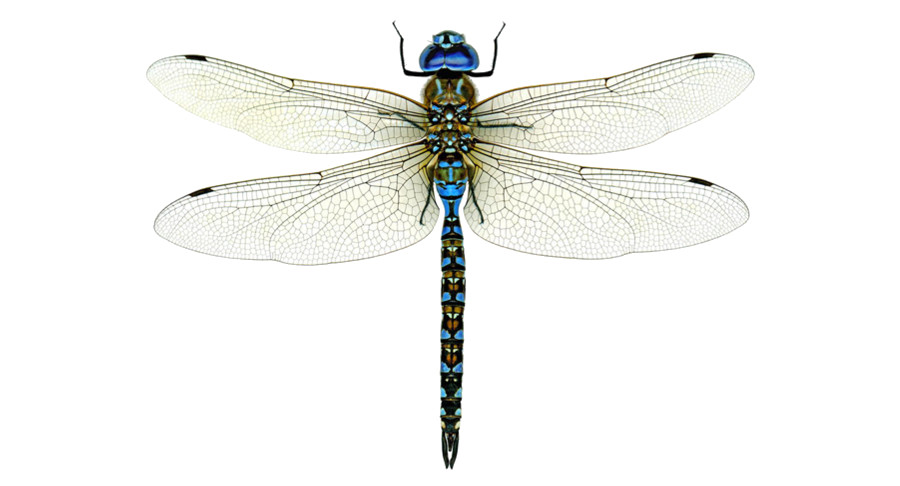
\includegraphics[width=\linewidth]{dragonfly.jpg}

\vspace{0.25 cm}
wings are not limbs
\end{center}

\column{0.35\linewidth}
\begin{center}
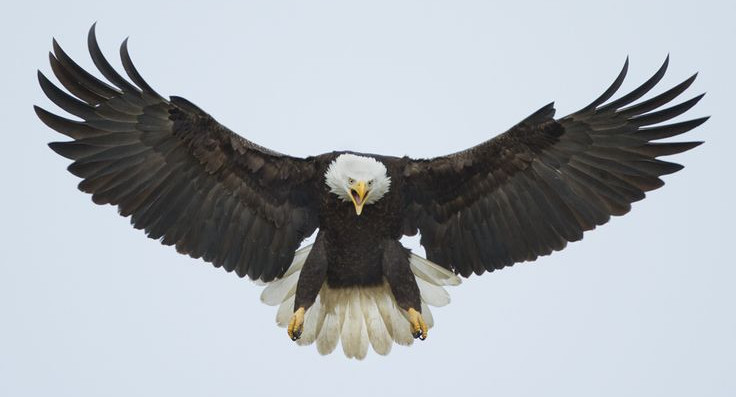
\includegraphics[width=\linewidth]{bird.jpg}

\vspace{0.25 cm}
wings are arms
\end{center}

\column{0.35\linewidth}
\begin{center}
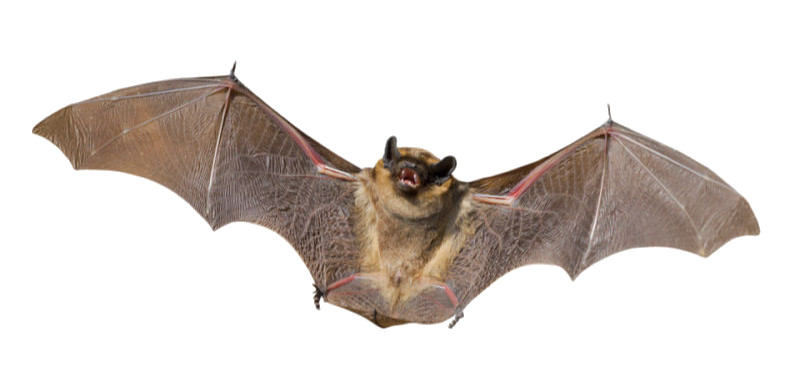
\includegraphics[width=\linewidth]{bat.jpg}

\vspace{0.25 cm}
wings are hands
\end{center}
\end{columns}
\end{frame}

\begin{frame}{Feature comparison: ROOT and Parquet}
\vspace{0.5 cm}
\begin{columns}[t]
\column{0.5\linewidth}
{\large \underline{ROOT}}

\begin{itemize}
\item Store individual C++ objects rowwise in TDirectories and large collections of C++ objects (or simple tables) rowwise or columnar in TTrees.
\item Can rewrite to the same file, like a database, but most users write once.
\item \textcolor{darkorange}{Selective reading of columns (same).}
\item \textcolor{darkorange}{Cluster/basket structure (same).}
\item Plain encodings, one level of depth (deeper structures are rowwise).
\item Compression codecs: gzip, lz4, lzma, \textcolor{gray}{zstd (under consideration)}
\end{itemize}

\column{0.5\linewidth}
{\large \underline{Parquet}}

\begin{itemize}
\item Only store large collections of language-independent, columnar objects. The whole Parquet file is like a single TTree.
\item Write once, producing an immutable artifact.
\item \textcolor{darkorange}{Selective reading of columns (same).}
\item \textcolor{darkorange}{Row group/page structure (same).}
\item Highly packed encodings, any level of depth (logarithmic scaling with depth).
\item Compression codecs: snappy, gzip, lzo, brotli, \textcolor{gray}{lz4, zstd (version 2.3.2)}
\end{itemize}
\end{columns}
\end{frame}

\begin{frame}{Implementation comparision: ROOT and Parquet (1)}
\vspace{0.5 cm}
\begin{columns}[t]
\column{0.5\linewidth}
{\large \underline{ROOT}}

\begin{itemize}
\item Metadata and search through the file starts with a header.

\item Header must be rewritten as objects (including baskets) accumulate.

\item Failure is partially recoverable, but writing is non-sequential.

\item Also facilitates rewriting (use as a database).
\end{itemize}

\column{0.5\linewidth}
{\large \underline{Parquet}}

\begin{itemize}
\item Metadata and search through the file starts with a footer.

\item Data are written sequentially and seek points are only written at the end.

\item Failure invalidates the whole file, but writing is sequential.

\item Parquet files are supposed to be immutable artifacts.
\end{itemize}
\end{columns}
\end{frame}

\begin{frame}{Implementation comparision: ROOT and Parquet (2)}
\vspace{0.5 cm}
\begin{columns}[t]
\column{0.5\linewidth}
{\large \underline{ROOT}}

\begin{itemize}
\item Layout of metadata and data structures are specified by streamers, which are saved to the same file.

\item Streamer mechanism has built-in schema evolution.

\item Data types are C++ types. \mbox{\hspace{5 cm}} \mbox{\hspace{5 cm}}

\item Objects in TTrees are specified by the same streamers.
\end{itemize}

\column{0.5\linewidth}
{\large \underline{Parquet}}

\begin{itemize}
\item Layout of metadata and data structures are specified by Thrift, an existing rowwise object specification.

\item Thrift has schema evolution. \mbox{\hspace{5 cm}}

\item Simple data types are described by a physical schema, related to external type systems by a logical schema.

\item Thrift for metadata, schemas for data--- no unification.
\end{itemize}
\end{columns}
\end{frame}

\begin{frame}{Implementation comparision: ROOT and Parquet (3)}
\vspace{0.5 cm}
\begin{columns}
\column{0.52\linewidth}
{\large \underline{ROOT}}

\begin{itemize}
\item Contiguous data array accompanied by:

\begin{itemize}
\item navigation array: pointers to the start of each variable-sized object.
\end{itemize}

\item Permits random access by entry index.
\end{itemize}

\column{0.52\linewidth}
{\large \underline{Parquet}}

\begin{itemize}
\item Contiguous data array accompanied by:
\begin{itemize}
\item definition levels: integers indicating depth of first {\tt\small null} in data; maximum for non-null data.
\item repetition levels: integers indicating depth of continuing sub-list, e.g.\ {\tt\small 0} means new top-level list.
\end{itemize}

\item Definition levels even required for non- nullable data, to encode empty lists.

\item Schema depth fixes maximum definition/repetition values, and therefore their number of bits.

\item Must be unraveled for random access.
\end{itemize}
\end{columns}
\end{frame}

\begin{frame}{Implementation comparision: ROOT and Parquet (4)}
\vspace{0.5 cm}
\begin{columns}
\column{0.5\linewidth}
{\large \underline{ROOT}}

\begin{itemize}
\item Data are simply encoded, by streamers or as basic C++ types (e.g.\ {\tt\small Char\_t, Int64\_t, float, double}).
\end{itemize}

\column{0.5\linewidth}
{\large \underline{Parquet}}

\begin{itemize}
\item Integers and booleans with known maxima are packed into the fewest possible bits.

\item Other integers are encoded in variable-width formats, e.g.\ 1~byte up to 127, 2~bytes up to 16511, zig-zagging for signed integers.

\item Dynamically switches between run length encoding and bit-packing.

\item Optional ``dictionary encoding,'' which replaces data with a dictionary of unique values and indexes into that dictionary (variable-width encoded).
\end{itemize}
\end{columns}
\end{frame}

\begin{frame}{Implementation comparision: ROOT and Parquet (5)}
\vspace{0.5 cm}
\begin{columns}
\column{0.5\linewidth}
{\large \underline{ROOT}}

\begin{itemize}
\item Granular unit of reading and decompression is a basket, which may be anywhere in the file (located by TKey).

\item Entry numbers of baskets {\it may} line up in clusters (controlled by {\tt\small AutoFlush}). Clusters are a convenient unit of parallelization.
\end{itemize}

\column{0.5\linewidth}
{\large \underline{Parquet}}

\begin{itemize}
\item Granular unit of reading and decompression is a page, which must be contiguous by column (similar to ROOT's {\tt\small SortBasketsByBranch}).

\item Entry numbers of columns (contiguous group of pages) {\it must} line up in row groups, which are the granular unit of parallelization.
\end{itemize}
\end{columns}
\end{frame}

\begin{frame}{}
\vspace{0.5 cm}
\begin{center}
\Huge \textcolor{darkblue}{File size comparisons}
\end{center}
\end{frame}

\begin{frame}{Parameters of the test (1)}
\vspace{0.35 cm}
\begin{description}
\item[Datasets:] 13 different physics samples in CMS NanoAOD.

\vspace{0.1 cm}
Non-trivial structure: variable length lists of numbers, but no objects.

\vspace{0.2 cm}
\item[ROOT:] version 6.12/06 (latest release)

\begin{itemize}
\item Cluster sizes: 200, 1000, 5000, 20\,000, 100\,000 events
\item Basket size: 32\,000 bytes (1~basket per cluster in all but the largest)
\item Freshly regenerated files in this ROOT version: {\tt\small GetEntry} from the CMS originals and {\tt\small Fill} into the datasets used in this study.
\end{itemize}

\item[Parquet:] C++ version 1.3.1 inside pyarrow-0.8.0 (latest release)

\begin{itemize}
\item Generated by ROOT $\to$ uproot $\to$ Numpy $\to$ pyarrow $\to$ Parquet, controlling array size so that Parquet row groups are identical to ROOT clusters, pages to baskets.
\item Parquet files preserve the complete semantic information of the original, we can read back same variable length lists of numbers.
\end{itemize}
\end{description}
\end{frame}

\begin{frame}{Parameters of the test (2)}
\vspace{0.4 cm}
The purpose of the ensemble of 13 physics samples is to vary probability distributions: e.g.\ Drell-Yan has a different muons-to-jets ratio than $t\bar{t}$.

\vspace{0.25 cm}
However, these samples also differ in total content (number of events, number of particles), which is not relevant to performance.

\vspace{0.25 cm}
Each {\it sample} is divided by its ``na\"ive size,'' obtained by saving as Numpy files:
\begin{itemize}
\item Each $n$ byte number in memory becomes an $n$ byte number on disk.
\item Each boolean in memory becomes 1 bit on disk (packed).
\item No compression, insignificant metadata ($<$1~kB per GB file).
\end{itemize}

\vspace{0.25 cm}
Different conditions (cluster sizes, compression cases) and formats (ROOT, Parquet) have the {\it same} normalization factor for the {\it same} sample.

\vspace{0.25 cm}
Normalized sizes above 1.0 are due to metadata and overhead; below 1.0 due to compression or packed encodings.
\end{frame}

\begin{frame}{Normalized file sizes versus cluster/row group size}
\vspace{-0.1 cm}
\small
\begin{columns}
\column{0.26\linewidth}
\begin{center}
\normalsize ROOT uncompressed

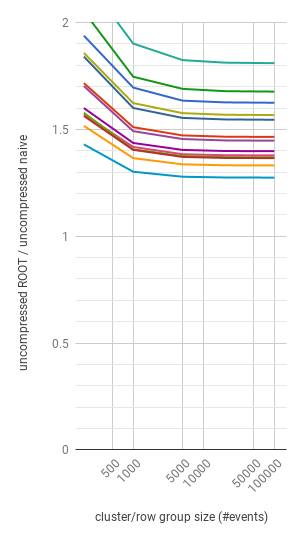
\includegraphics[width=\linewidth]{root-none.png}
\end{center}
\column{0.26\linewidth}
\begin{center}
\normalsize Parquet uncompressed

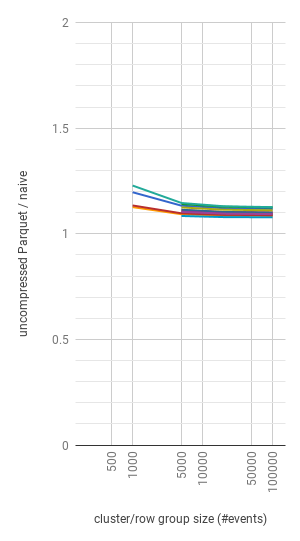
\includegraphics[width=\linewidth]{parquet-none.png}
\end{center}
\column{0.26\linewidth}
\begin{center}
\normalsize ROOT gzip

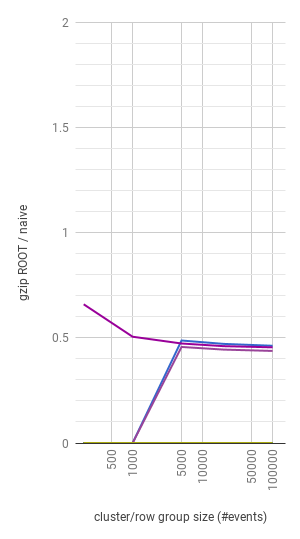
\includegraphics[width=\linewidth]{root-gzip.png}
\end{center}
\column{0.26\linewidth}
\begin{center}
\normalsize Parquet gzip

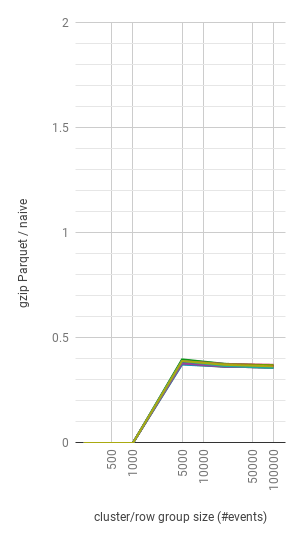
\includegraphics[width=\linewidth]{parquet-gzip.png}
\end{center}
\end{columns}

\vspace{0.25 cm}
Uncompressed Parquet is smaller and less variable than ROOT, but gzip-compressed are similar.
\end{frame}

\begin{frame}{Parquet's dictionary encoding is like a compression algorithm}
\begin{columns}
\column{0.26\linewidth}
\begin{center}
\mbox{\hspace{3 cm}}
ROOT gzip

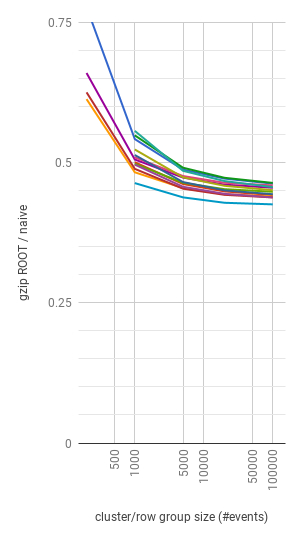
\includegraphics[width=\linewidth]{root-gzip-2.png}
\end{center}
\column{0.26\linewidth}
\begin{center}
Parquet uncompressed
with dict-encoding

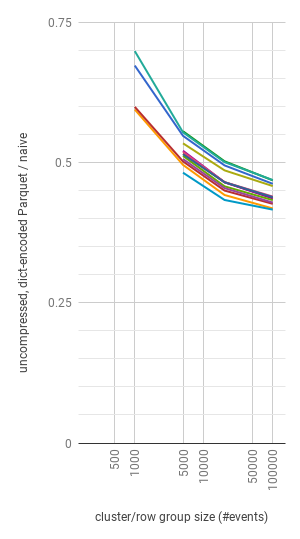
\includegraphics[width=\linewidth]{parquet-dict.png}
\end{center}
\column{0.26\linewidth}
\begin{center}
\mbox{\hspace{3 cm}}
ROOT lzma

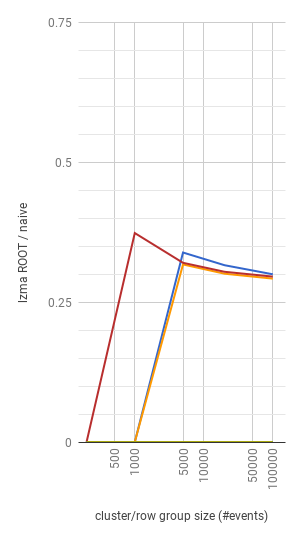
\includegraphics[width=\linewidth]{root-lzma.png}
\end{center}
\column{0.26\linewidth}
\begin{center}
\mbox{\hspace{3 cm}}
Parquet gzip

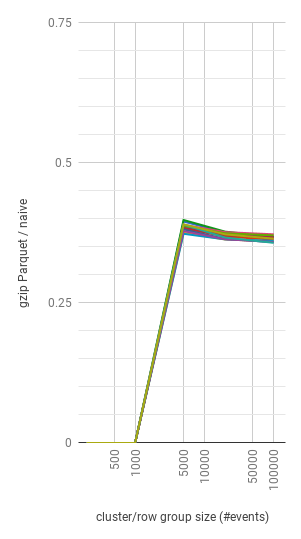
\includegraphics[width=\linewidth]{parquet-gzip-2.png}
\end{center}
\end{columns}
\end{frame}

\begin{frame}{Effect of NanoAOD's many boolean branches}
\vspace{0.35 cm}
$601+21$ of NanoAOD's $955$ branches are booleans (named {\tt\small HLT\_*} and {\tt\small Flag\_*}), which unnecessarily inflate the uncompressed ROOT size (8 bytes per boolean).

\vspace{0.25 cm}
Highest cluster/row group (100\,000 events), average and \underline{standard deviation} sizes:

\renewcommand{\arraystretch}{1.2}

\begin{center}
\begin{tabular}{r c c | c c}
                    & \multicolumn{2}{c}{all branches} & \multicolumn{2}{c}{without trigger} \\
                    & ROOT            & Parquet         & ROOT            & Parquet          \\\hline
uncompressed        & $^{\textcolor{white}{*}}1.48 \pm 0.16^{\textcolor{white}{*}}$ & $^{\textcolor{white}{*}}1.10 \pm 0.02^{\textcolor{white}{*}}$ & $1.32 \pm 0.11$ & $^{\textcolor{white}{*}}1.10 \pm 0.02^*$  \\
dictionary encoding &                 & $0.44 \pm 0.02$ &                 & $0.42 \pm 0.01$  \\
lz4                 & $0.60 \pm 0.03$ &                 & $0.58 \pm 0.03$ &                  \\
gzip                & $0.45 \pm 0.01$ & $0.36 \pm 0.01$ & $^{\textcolor{white}{*}}0.45 \pm 0.01^*$ & $0.37 \pm 0.01$  \\
lzma                & $0.30 \pm 0.01$ &                 & $0.29 \pm 0.01$ &                  \\
\end{tabular}
\end{center}

\vspace{-0.1 cm}
\hfill {\scriptsize ($^*$not copy-paste errors)}

\vspace{0.2 cm}
The triggers alone are not responsible for the large ROOT file sizes (and variance).
\end{frame}

\begin{frame}{Effect of dropping offset arrays (new TIOFeatures)}
\vspace{0.35 cm}
Last year, we predicted 10--30\% improvements if we drop offset arrays, depending on compression algorithm (lzma had the least to gain, lz4 the most).

\vspace{0.25 cm}
Highest cluster/row group (100\,000 events), average and \underline{standard deviation} sizes:

\renewcommand{\arraystretch}{1.2}

\begin{center}
\begin{tabular}{r c c c}
                    & ROOT default    & ROOT no offsets & Parquet         \\\hline
uncompressed        & $1.48 \pm 0.16$ & $1.20 \pm 0.07$ & $1.10 \pm 0.02$ \\
gzip                & $0.45 \pm 0.01$ & $0.35 \pm 0.01$ & $0.36 \pm 0.01$ \\
lzma                & $0.30 \pm 0.01$ & $0.27 \pm 0.01$ &                 \\
lz4                 & $0.60 \pm 0.03$ & $0.41 \pm 0.01$ &                 \\
dictionary encoding &                 &                 & $0.44 \pm 0.02$ \\
\end{tabular}
\end{center}

\vspace{0.25 cm}
Dropping offset arrays is a little better than predicted and brings ROOT-gzip exactly in line with Parquet-gzip. However, ROOT-lz4 is about the same as {\it uncompressed} Parquet with dictionary encoding.
\end{frame}

\begin{frame}{}
\vspace{0.5 cm}
\begin{center}
\Huge \textcolor{darkblue}{Throughput comparisons}
\end{center}
\end{frame}

\begin{frame}{ROOT reading rate / Parquet reading rate}
\vspace{-0.15 cm}

\begin{columns}
\column{0.35\linewidth}
\begin{center}
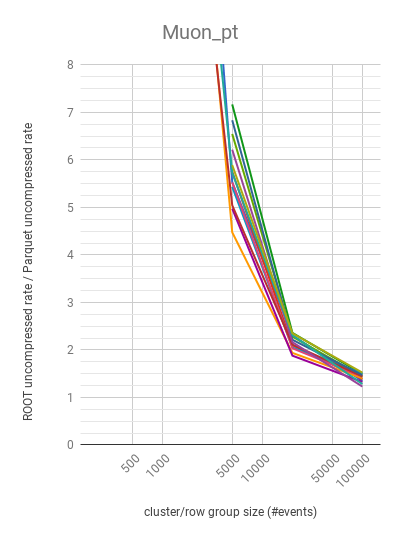
\includegraphics[width=\linewidth]{root-none-parquet-none-Muon_pt.png}
\end{center}
\column{0.35\linewidth}
\begin{center}
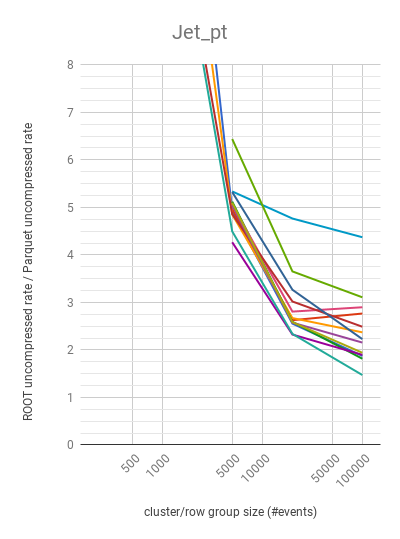
\includegraphics[width=\linewidth]{root-none-parquet-none-Jet_pt.png}
\end{center}
\column{0.35\linewidth}
\begin{center}
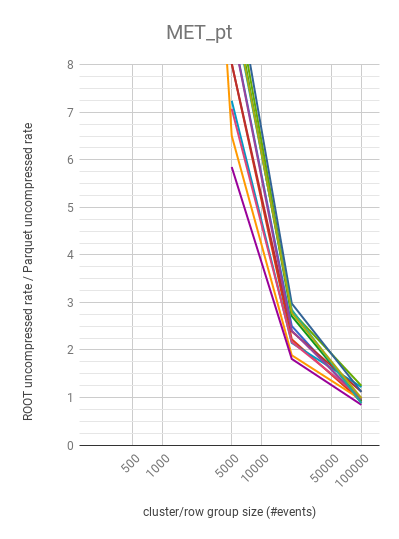
\includegraphics[width=\linewidth]{root-none-parquet-none-MET_pt.png}
\end{center}
\end{columns}

\vspace{0.25 cm}
ROOT is much faster than Parquet-C++ for small cluster/row group sizes, but the difference levels out at high cluster/row group sizes.
\end{frame}

\begin{frame}{ROOT reading rate / Parquet reading rate: both gzipped}
\vspace{-0.15 cm}

\begin{columns}
\column{0.35\linewidth}
\begin{center}
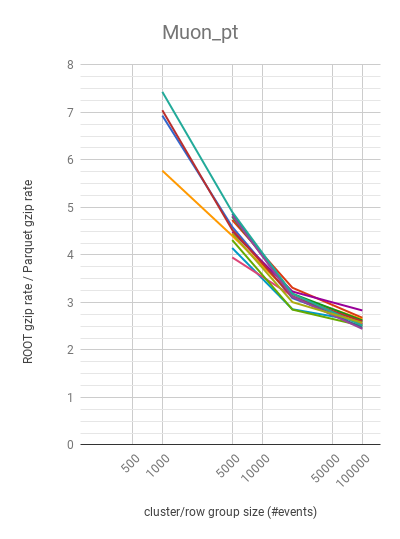
\includegraphics[width=\linewidth]{root-gzip-parquet-gzip-Muon_pt.png}
\end{center}
\column{0.35\linewidth}
\begin{center}
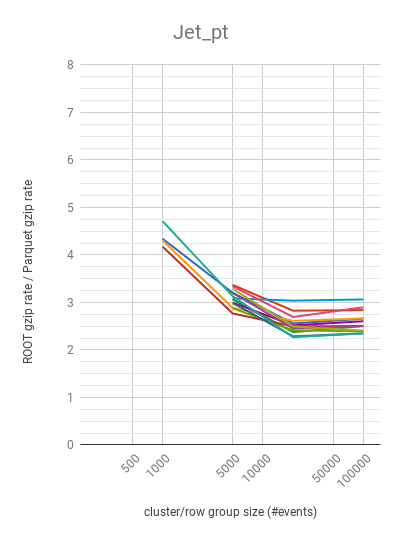
\includegraphics[width=\linewidth]{root-gzip-parquet-gzip-Jet_pt.png}
\end{center}
\column{0.35\linewidth}
\begin{center}
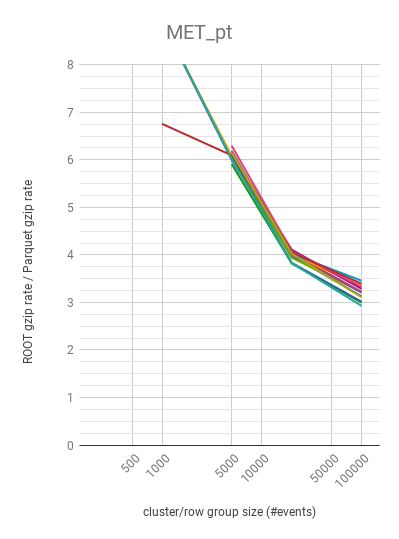
\includegraphics[width=\linewidth]{root-gzip-parquet-gzip-MET_pt.png}
\end{center}
\end{columns}

\vspace{0.25 cm}
The slope with respect to cluster/row group size is less pronounced when both are gzipped, but still ROOT is several times faster.
\end{frame}

\begin{frame}{ROOT reading rate (lz4) / Parquet reading rate (dict-encoded)}
\vspace{-0.15 cm}

\begin{columns}
\column{0.35\linewidth}
\begin{center}
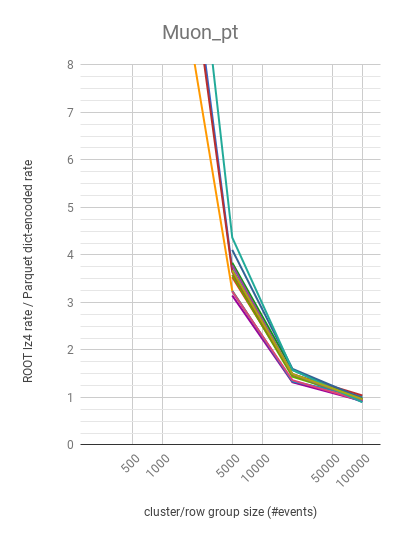
\includegraphics[width=\linewidth]{root-lz4-parquet-dict-Muon_pt.png}
\end{center}
\column{0.35\linewidth}
\begin{center}
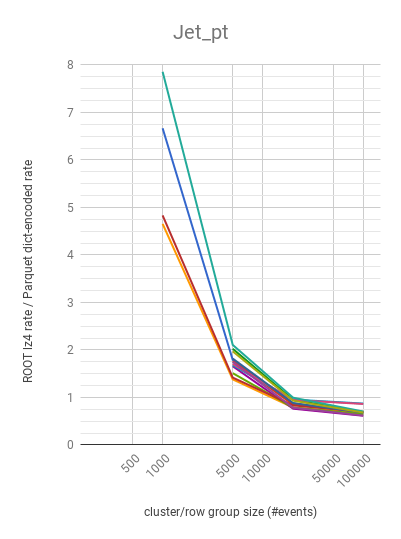
\includegraphics[width=\linewidth]{root-lz4-parquet-dict-Jet_pt.png}
\end{center}
\column{0.35\linewidth}
\begin{center}
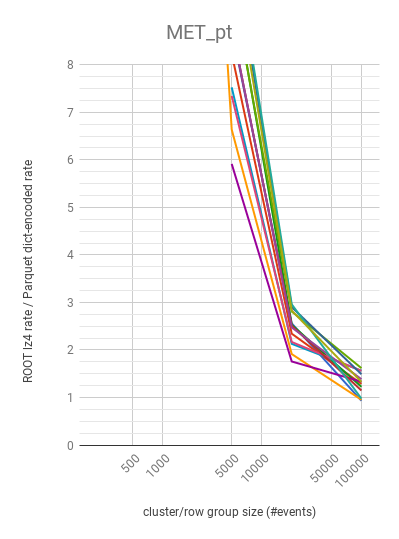
\includegraphics[width=\linewidth]{root-lz4-parquet-dict-MET_pt.png}
\end{center}
\end{columns}

\vspace{0.25 cm}
Decoding lz4 in ROOT is about as fast as decoding Parquet's dictionary encoding (given large cluster/row group sizes), so there's no size vs speed advantage.
\end{frame}

\begin{frame}{Throughput summary}
\vspace{0.35 cm}
Highest cluster/row group (100\,000 events), average and \underline{standard deviation} times to read 10 branches (seconds):

\renewcommand{\arraystretch}{1.2}

\begin{center}
\begin{tabular}{r c c | c c}
                    & \multicolumn{2}{c}{ROOT} & \multicolumn{2}{c}{Parquet} \\
                    &  cold cache    &  warm cache    & cold cache    & warm cache    \\\hline
uncompressed        &  $0.6 \pm 0.2$ &  $0.4 \pm 0.2$ & $1.1 \pm 0.3$ & $1.0 \pm 0.3$ \\
gzip                &  $1.6 \pm 0.5$ &  $1.4 \pm 0.4$ & $3.1 \pm 0.9$ & $3.1 \pm 0.9$ \\
lzma                & $12.2 \pm 3.7$ & $12.1 \pm 3.7$ &               &               \\
lz4                 &  $1.4 \pm 0.4$ &  $1.3 \pm 0.4$ &               &               \\
dictionary encoding &                &                & $1.0 \pm 0.3$ & $1.0 \pm 0.3$ \\
\end{tabular}
\end{center}

\vspace{0.25 cm}
For large cluster/row groups, ROOT 6.12/06 is twice as fast as Parquet-C++ 1.3.1.
\end{frame}

\begin{frame}{Summary: Parquet's encodings yield smaller and slower files}
\vspace{0.15 cm}\Large
\begin{columns}
\column{0.7\linewidth}
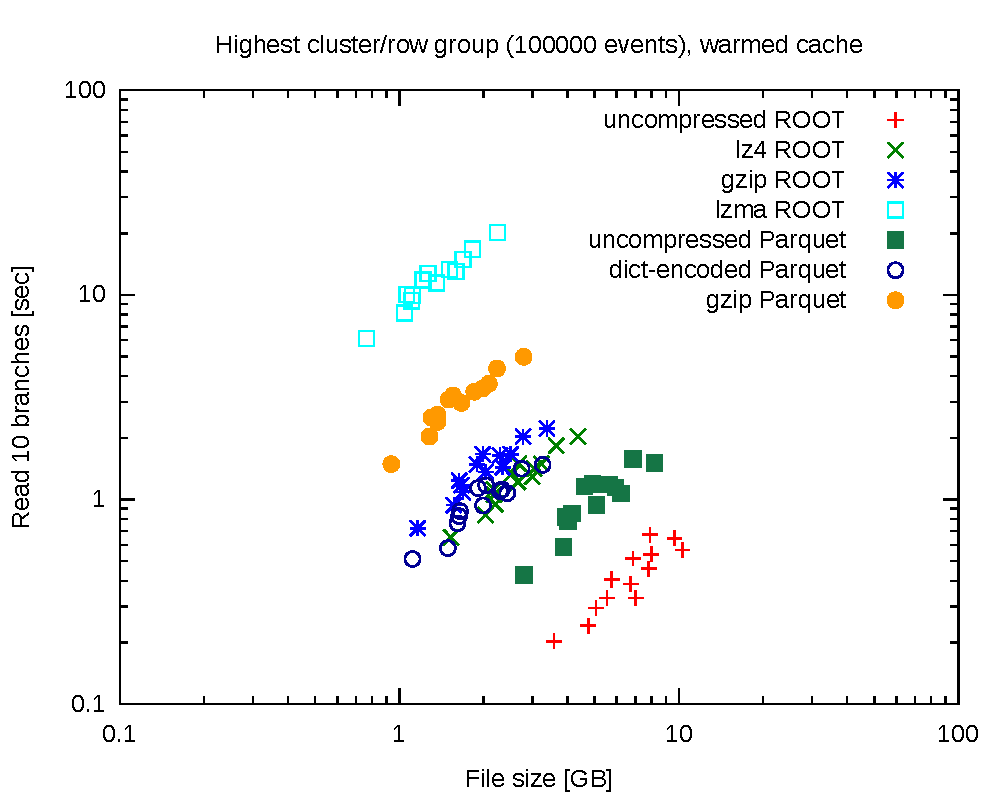
\includegraphics[width=\linewidth]{root-parquet-size-throughput.pdf}

\column{0.3\linewidth}
\ldots like compression
\end{columns}
\end{frame}

\end{document}
